\section{Demonstration}

\subsection{Interface Overview}

\begin{frame}{Interface Overview}
  \begin{figure}
    \begin{annotatedFigure}
      {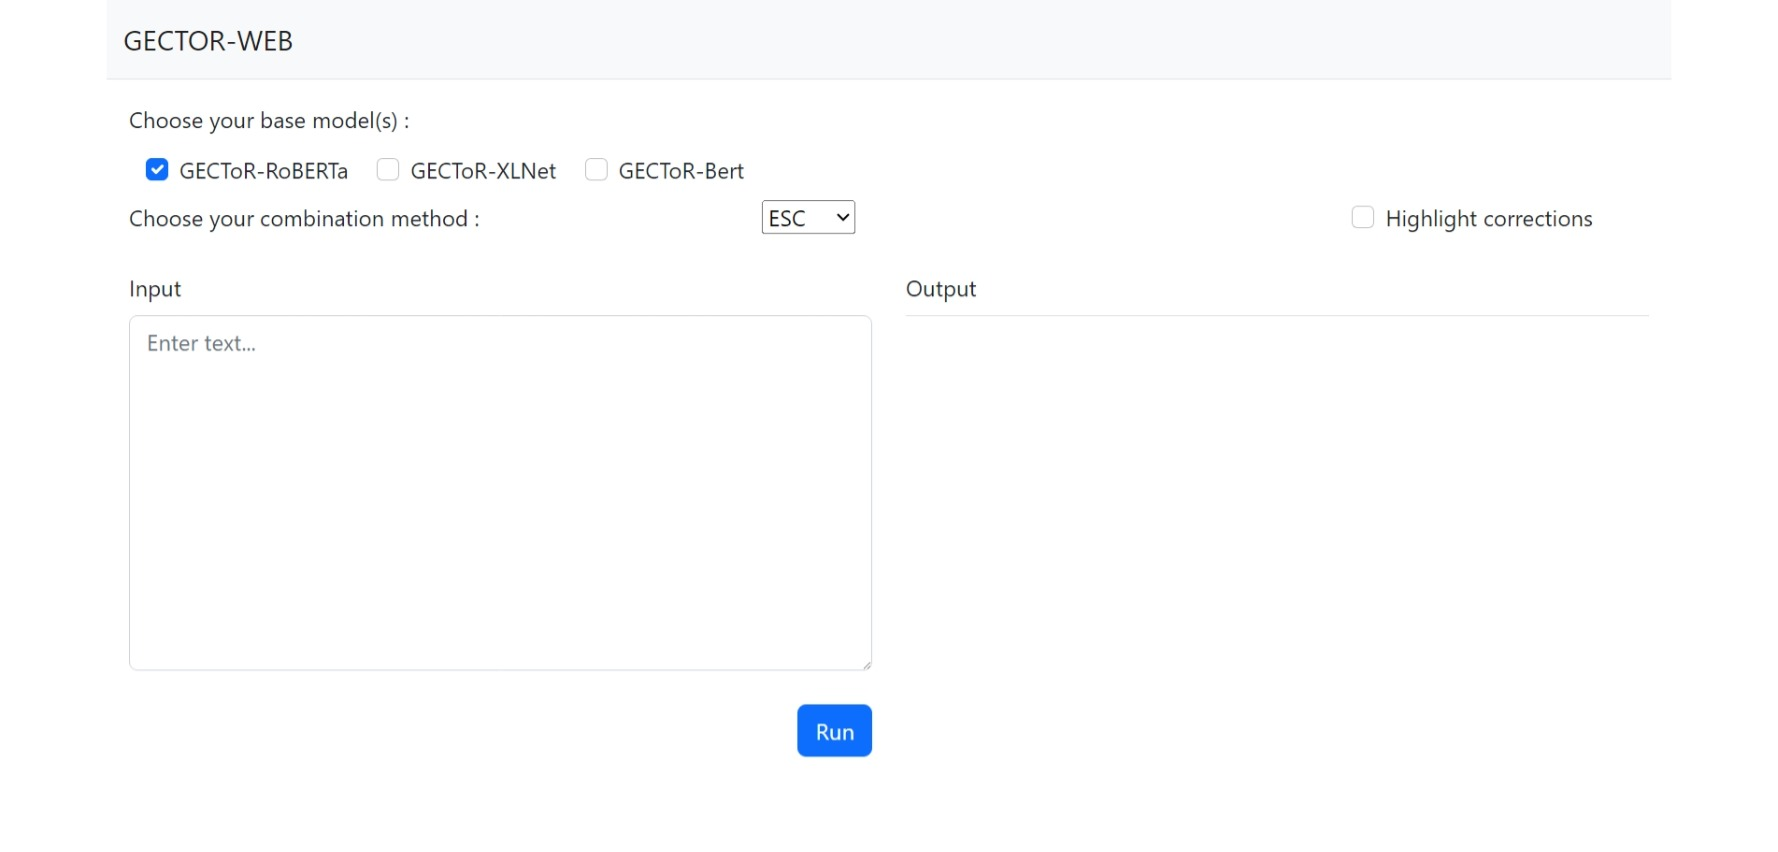
\includegraphics[width=0.85\textwidth]{home}}
      \pause
      \annotatedFigureBox{0.0905,0.7727}{0.4305,0.8393}{i}{0.4305,0.8393}%tr
      \pause
      \annotatedFigureBox{0.434,0.7266}{0.5105,0.8003}{ii}{0.5105,0.8003}%tr
      \pause
      \annotatedFigureBox{0.7615,0.7308}{0.9195,0.7934}{iii}{0.9195,0.7934}%tr
      \pause
      \annotatedFigureBox{0.1285,0.3489}{0.4595,0.6243}{iv}{0.4595,0.6243}%tr
      \pause
      \annotatedFigureBox{0.574,0.2591}{0.8665,0.6118}{v}{0.8665,0.6118}%tr
    \end{annotatedFigure}
    \caption{The User Interface of GecWeb.}
  \end{figure}

  \note<1>{
    The interface of GecWeb consists of five components.
  }

  \note<2>{
    The first component is the base model selection.

    If the user chooses more than one base model, GecWeb will run a system combination method based on the combination method selected.
  }

  \note<3>{
    Next is the combination method selection.
    If the user only chooses one base system, the selected combination method is ignored.
  }

  \note<4>{
    The third component is the output mode.

    User can choose to highlight the corrections by selecting the ``Highlight corrections'' box to, as the name suggests, highlight the corrections in the output text.

    Additionally, it will display simple a explanations to help language learners understand their mistakes better.
  }

  \note<5>{
    The user is then put the text they want to correct in the input text box and clicks the run button.
  }

  \note<6>{
    The corrected text will then be displayed in the last component, the output text box.
  }
\end{frame}

\subsection{GecWeb Demo}

\begin{frame}{Access the Website}
  \centering

  {
    \Large \textbf{Visit GecWeb at:}
    \href{https://gratefully-wise-redfish.ngrok-free.app}{\textcolor{blue}{https://gratefully-wise-redfish.ngrok-free.app}}
  }

  \vspace{1cm}

  \qrcode[height=4cm]{https://gratefully-wise-redfish.ngrok-free.app}

\end{frame}

\note{
  Before we proceed to the demonstration, you can try GecWeb yourself by visiting the website at the link shown on the screen or scanning the QR code.

  Don't mind the weird url though, I get it from a free hosting service.
  Because I am too broke to afford my own domain.
  That url is screaming ``I'm broke''.
}

\begin{frame}{GecWeb Demo (Desktop)}
  \begin{figure}
    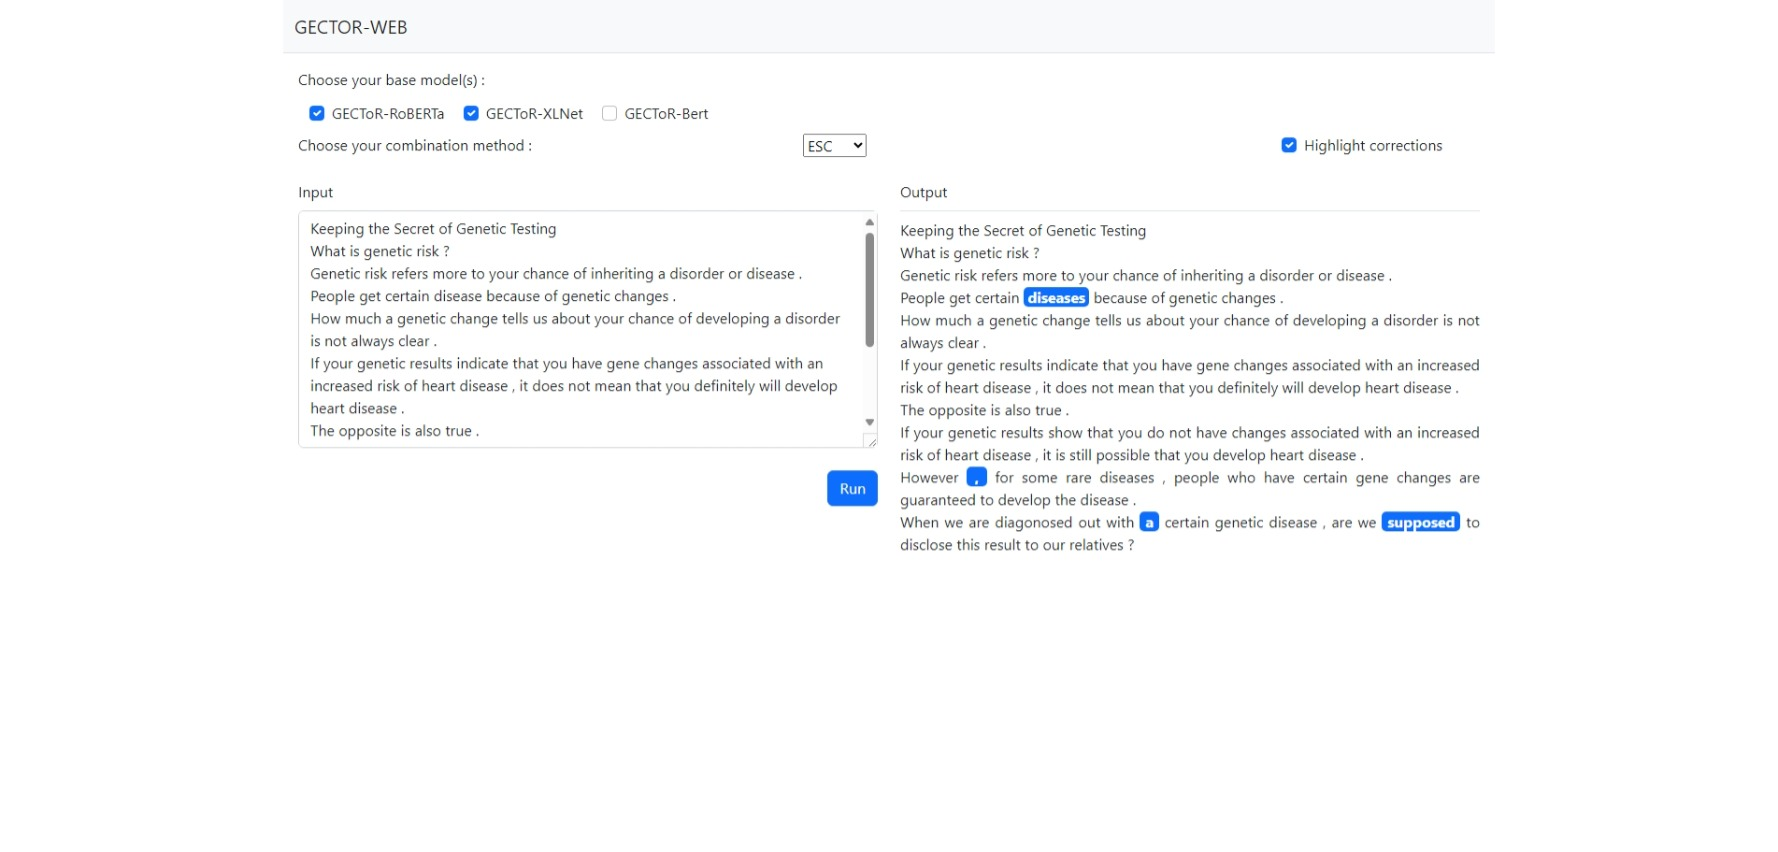
\includegraphics[width=0.9\textwidth]{highlight}
    \caption{GecWeb running on a desktop browser with correction highlights enabled.}
  \end{figure}
\end{frame}

\begin{frame}{GecWeb Demo (Desktop)}
  \begin{figure}
    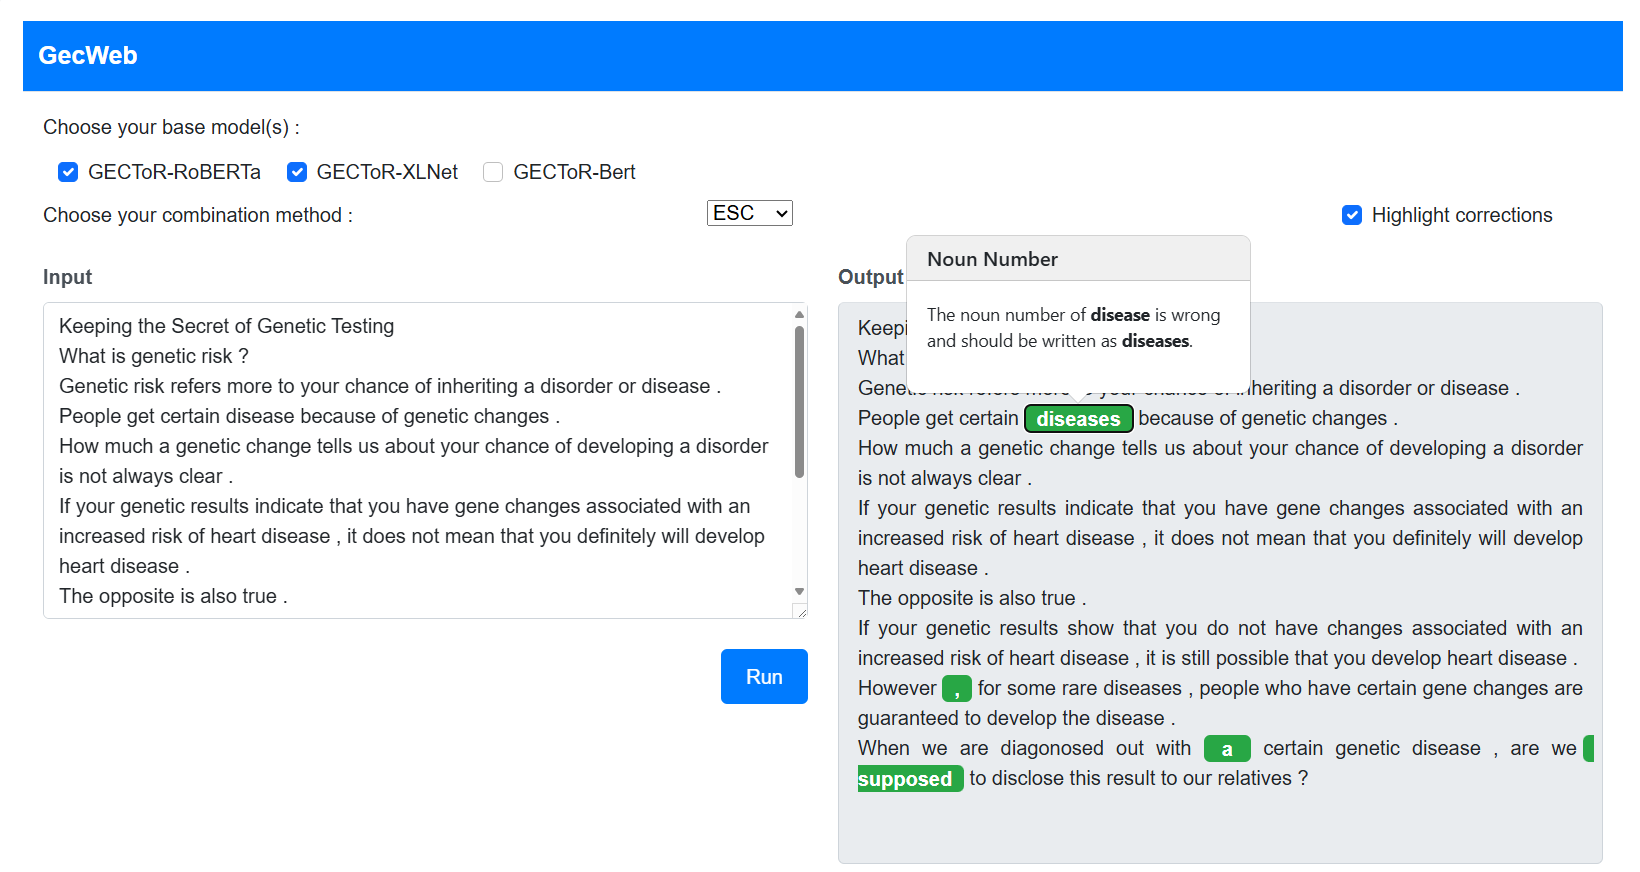
\includegraphics[width=0.8\textwidth]{highlight+note}
    \caption{GecWeb running on a desktop browser with notes about the corrections.}
  \end{figure}
\end{frame}

\begin{frame}{GecWeb Demo (Mobile)}
  \begin{figure}
    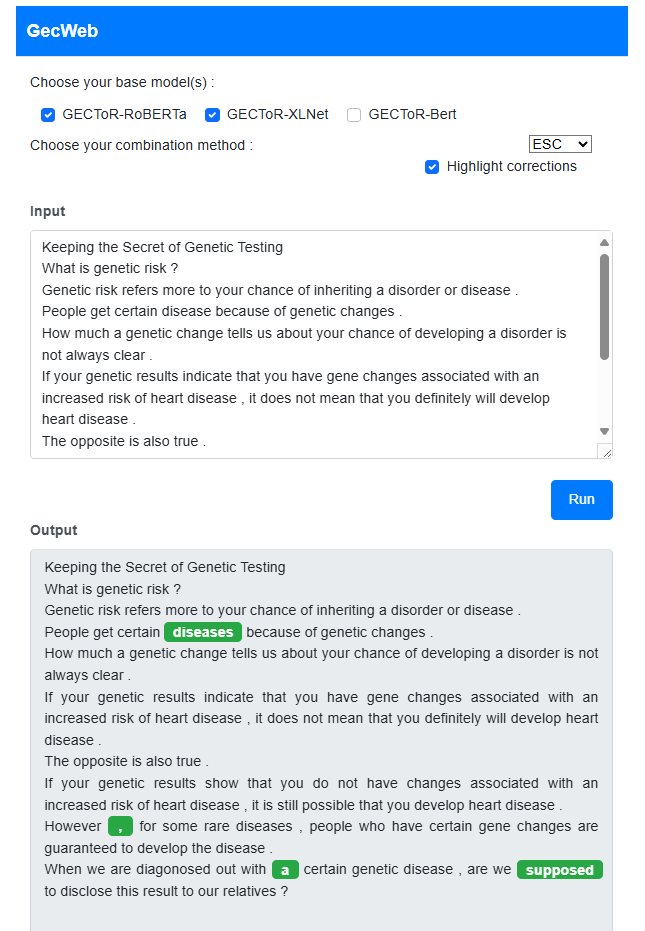
\includegraphics[height=0.75\textheight]{mobile}
    \caption{GecWeb running on a mobile phone.}
  \end{figure}
\end{frame}
